\input{beamer.macros}
\usepackage[english]{babel}
\usepackage{tikz}
\newcommand{\fadeitem}[2]{\item[]\uncover<#1>{#2}}
\title{Validating Neighborhoods}
\author{Forest Gregg}
\begin{document}
\mode*
\maketitle

\mode<all>{
\fullscreenimage{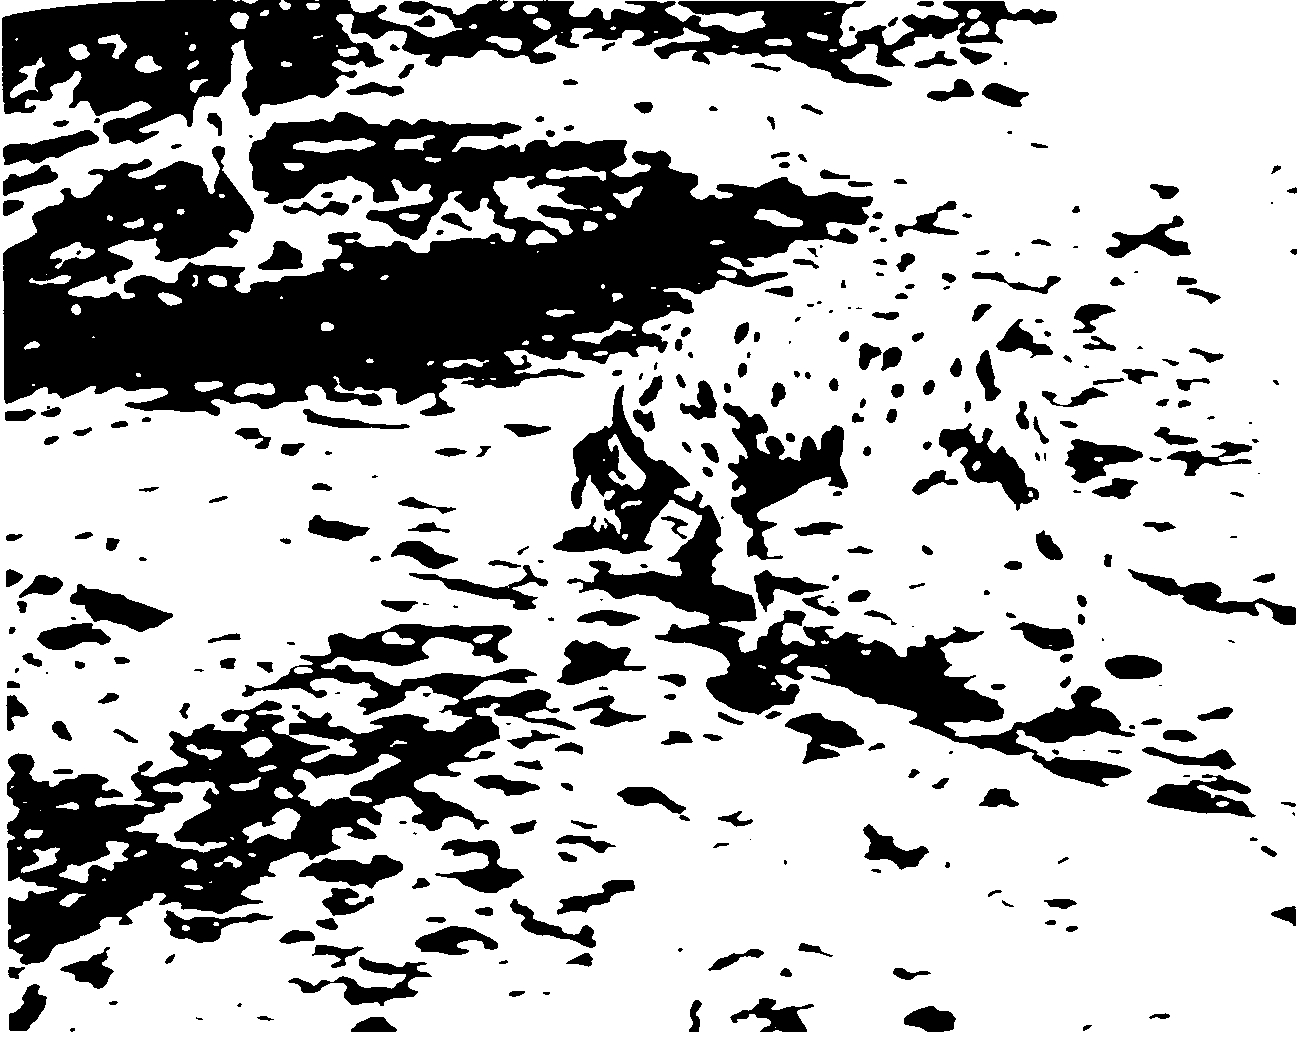
\includegraphics[width=\paperwidth]{./presentation_images/dog-park-big.jpg}}
}

\mode<all>{
\blackout{}
}  

\section{Introduction}
Today, I'd like to talk to you about a basic problem for social
research and some ideas about how we might respond. This is early
work, so I am going keep my presentation to 30 minutes so we have time
for a discussion.

So, here's the problem. In the social sciences, most of us study
aggregate things. Like class, status, party, social movements, or a
market. In order to get on with that studying, we have to say what
part of the world /is/ the thing we are studying.

If you want to study organizations, you have to decide what set of
entities and interactions are part of a particular organization and
which are not.

\mode<all>{
\fullscreenimage{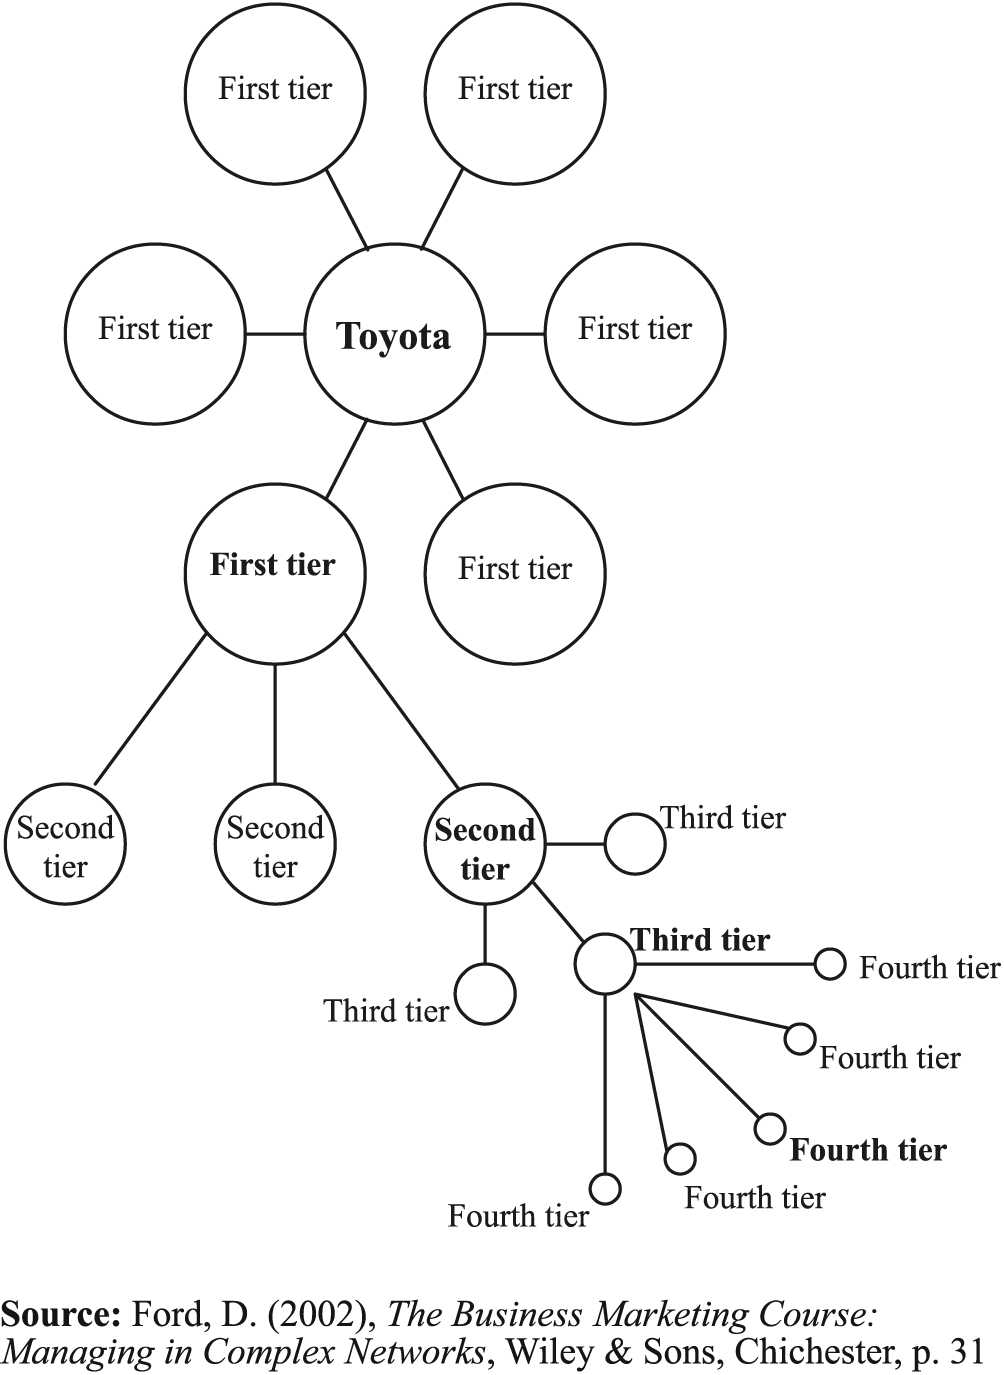
\includegraphics[height=\paperheight]{./presentation_images/toyotaSupply.png}}
}

If you want to study social movements, you have to decide how who is
and is not part of the movement?

\mode<all>{
\fullscreenimage{
\includegraphics[width=\paperwidth]{./presentation_images/99-percent.jpg}}
}

If you are studying scientific collaboration networks, you have to decide what counts as a collaboration. Is it co-authorship?

\mode<all>{
\fullscreenimage{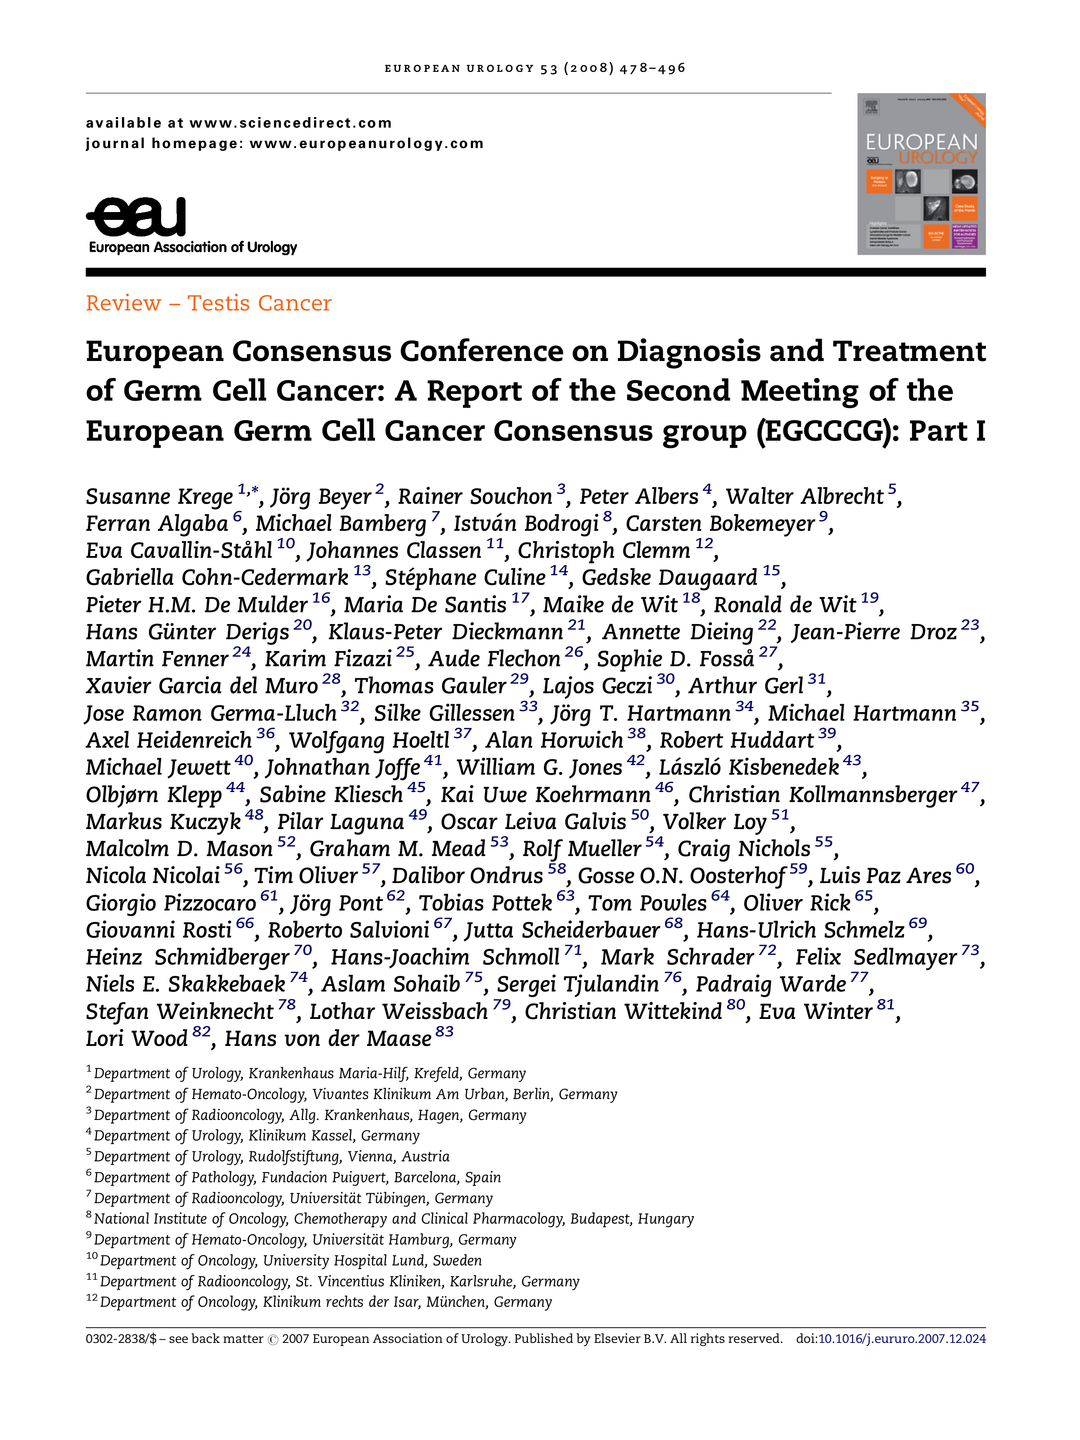
\includegraphics[height=\paperheight]{./presentation_images/many-author.png}}
}

\mode<all>{
\blackout{}
}  

To do empirical research about these social things we /have/ to divide
up the world. But, if we do that badly, then no degree of care of
observation or sophistication of technique can save us from drawing
wrong conclusions about the thing that we started out to understand.

So, how do we make sure we are not doing that? If we have to draw some boundaries, then 

\begin{frame}
\begin{center}
How do we know that we have gotten the boundaries right?
\end{center}
\end{frame}

Now, some of you are probably thinking -- it depends upon what we want
'right' to mean. I completely agree. I have some ideas, but I want
your help with that problem.

I think we may do better if we review a concrete case. If we look at
how some smart people smart people have tried to find good boundaries
for a particular kind of thing; that may be helpful to think with.

So, let's consider the neighborhood, and even more concretely, let's
consider how social scientists have attempted to identify the
neighborhoods of Chicago. Since the 1920s, once a generation somebody
takes on this task, usually pretty innocent of preceding efforts.
While that kind of forgetting may be bad for cumulative social
science, but it is good for our conversation today because it probably
contributed to a wider variety of approaches we can consider.

In my reading, it looks like there were four general approaches:

\begin{frame}
\begin{itemize}{}
\fadeitem{1}{Squinting at maps}
\pause
\fadeitem{2}{Hand-tuned clustering of maps}
\pause
\fadeitem{3}{Asking people to make the maps for us}
\pause 
\fadeitem{4}{Predicting neighborhoods}
\end{itemize}
\end{frame}

\section{Squinting}
{
\setbeamercovered{default}
\begin{frame}
\begin{itemize}{}
\item[] Squinting at maps
\item[] \color{gray}{Hand-tuned clustering of maps}
\item[] \color{gray}{Asking people to make the maps for us}
\item[] \color{gray}{Predicting neighborhoods}
\end{itemize}
\end{frame}
}


\mode<all>{
\fullscreenimage{\includegraphics[height=\paperheight]{../scientific_segments/social_base_chicago_bw_large.png}}
}
\mode<all>{
\fullscreenimage{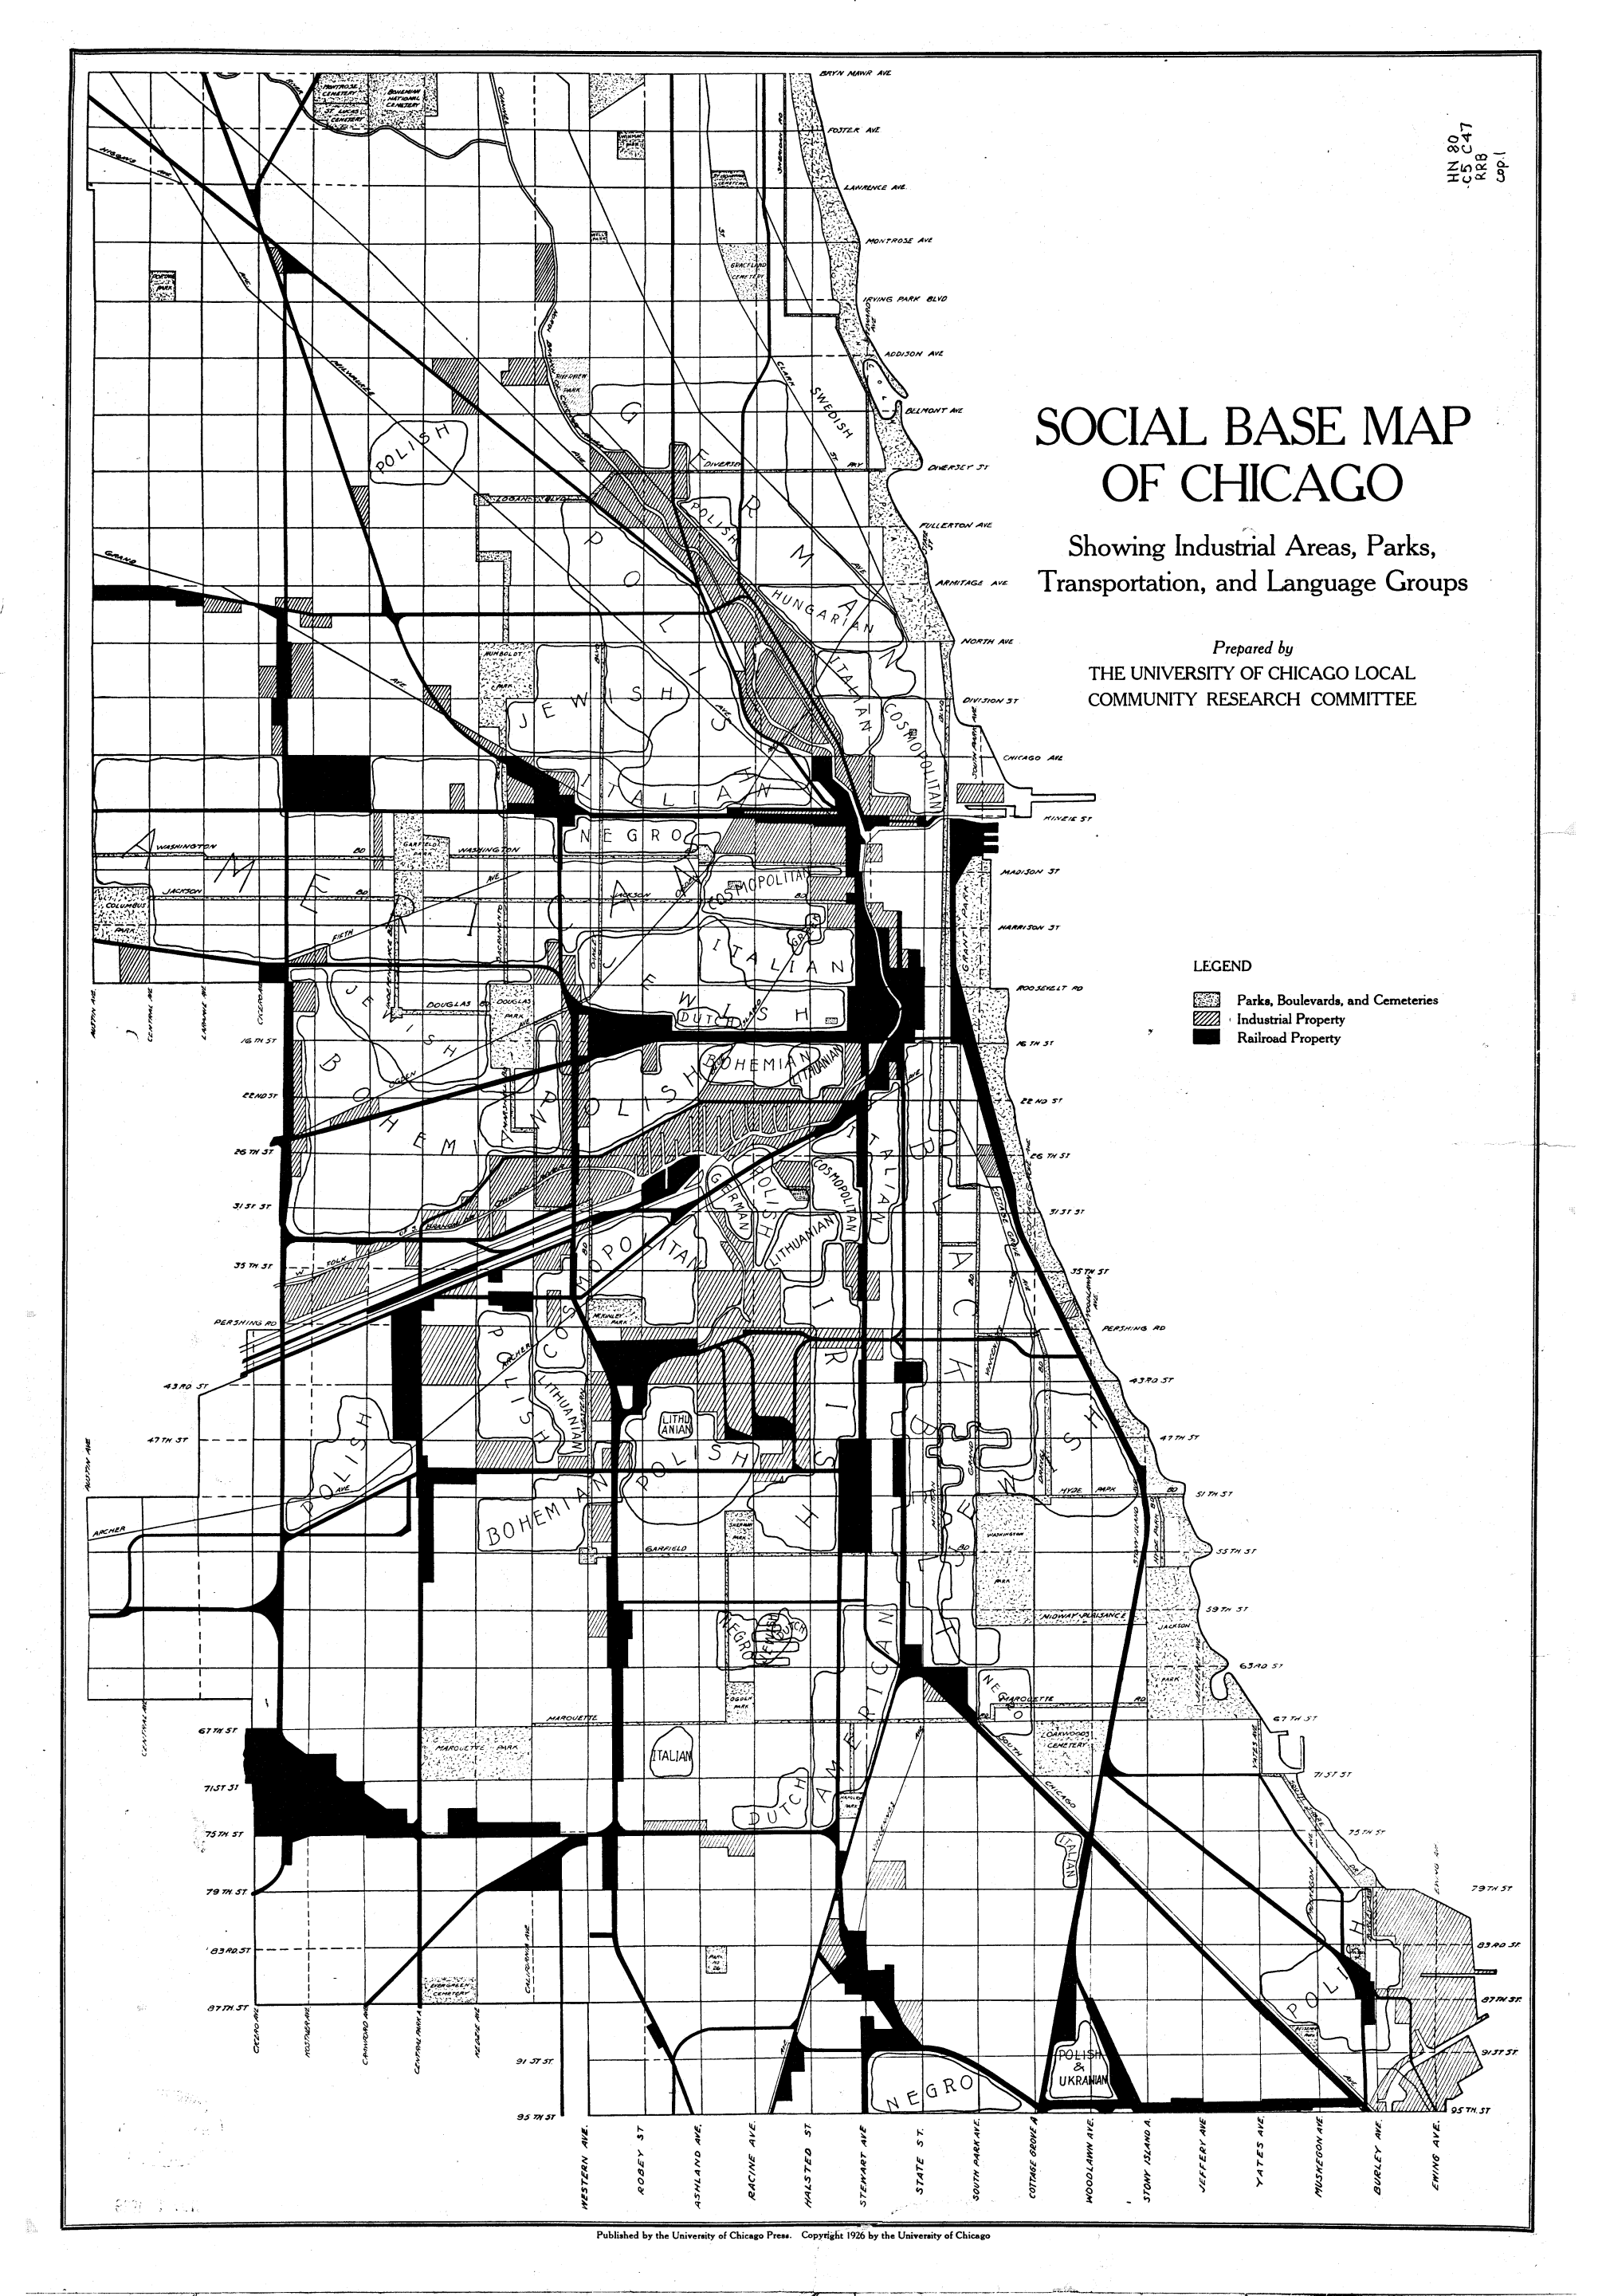
\includegraphics[height=\paperheight]{./preentation_images/output-0.png}}
}
\mode<all>{
\fullscreenimage{\includegraphics[height=\paperheight]{./preentation_images/output-1.png}}
}
\mode<all>{
\fullscreenimage{\includegraphics[height=\paperheight]{./preentation_images/output-2.png}}
}
\mode<all>{
\fullscreenimage{\includegraphics[height=\paperheight]{./preentation_images/output-3.png}}
}
\mode<all>{
\fullscreenimage{\includegraphics[height=\paperheight]{./preentation_images/output-4.png}}
}
\mode<all>{
\fullscreenimage{\includegraphics[height=\paperheight]{./preentation_images/output-5.png}}
}
\mode<all>{
\fullscreenimage{\includegraphics[height=\paperheight]{./preentation_images/output-6.png}}
}
\mode<all>{
\fullscreenimage{\includegraphics[height=\paperheight]{./preentation_images/output-7.png}}
}
\mode<all>{
\fullscreenimage{\includegraphics[height=\paperheight]{./preentation_images/output-8.png}}
}
\mode<all>{
\fullscreenimage{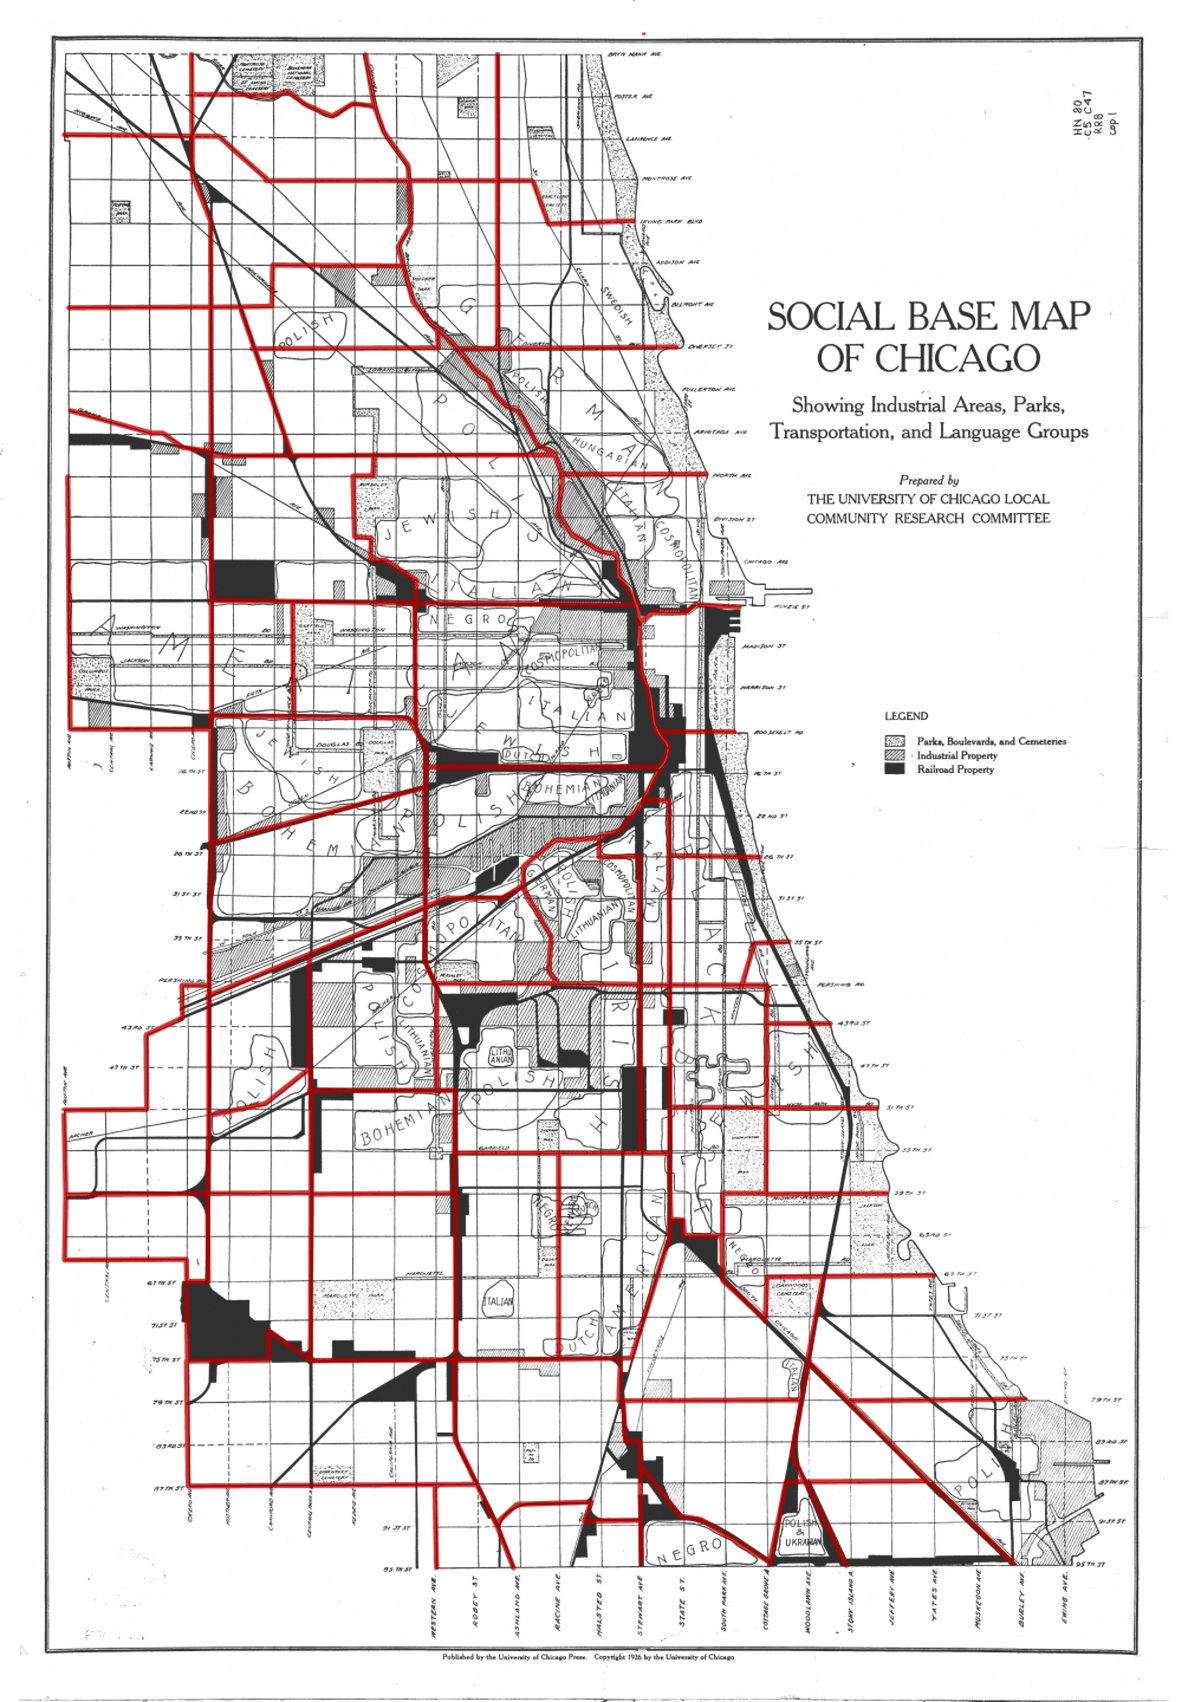
\includegraphics[height=\paperheight]{./preentation_images/output-9.png}}
}


In the 1920s, Ernest Burgess of the Department of Sociology at the
University of Chicago, had a map made of Chicago that showed the
rivers and canals, major street's, rail lines, parks, and industrial
areas. This was map was the a preliminary stage of a grand research
project that aimed to understand the principles behind the physical
growth of the fastest growing metropolis in the world, and the second
biggest city in the country.

Burgess saw that growth as driven by a very simple dynamic. Retailers,
manufacturers, and residents were all trying to minimize travel or
trucking costs.  The center of the city, the place of the minimum
average distance to any other part of the city, should therefore have
the most expensive land, and the price of land should fall with
distance from the center.  This price gradient should, in turn, sort
out the distribution of land uses. Retailers benefited most from
centrality, to the central district should be a commercial
zone. Manufacturers would be close by, and then residential
districts. As the city grew, the gradient of prices would shift
upwards, and the central commercial district would expand int to
manufacturing, and the manufacturing would take over residential
districts.

Even with a few more wrinkles, the theory was very simple and it
seemed to really explain the development of Chicago very well at a
rough level. However, the theory was silent about how uses of land
were distributed within a band of land prices. We know where to expect
a department store versus a warehouse, but why are all Germans on the
Northsdie of the river and all the Irish on the South?

For Burgess, there were two 




for Burgess, the competition for land was within any zone of land price, 

while the theory could tell you where you should expect to see a department store even in flat Chicago, Euclidean distance is not a very
good proxy for travel time. There are the various branches of the river, a

To make more precise predictions, Burgess appreciated that he
needed to do two things. First, 







the This bid up the cost of land, such tbenefited differentially from 



, a city that had grown from 

Burgess saw these large physical  

If we get the boundaries of these things wrong, then our
  observations are invalid.





 scholar  hase made without real eng usually without really knowing about the previo

THis history attempts to scientifically
define the neighborhoods of Chicago

















Last week, Jacob Foster showed us the network diagram of Wayne
Zachary's famous karate club, which had been divided into
'communities' by the X algorithm. 

\note{Read Wayne Zachary's famous paper, get image from Jacob, and
  figure out which algorithm produced that partition} 

% \mode<all>{
% \fullscreenimage{./presentation_images/karate.jpg}
% }



\testframe{}



For me, when I look at this picture, I have a feeling of
understanding. It looks to me like the algorithm uncovered a real
pattern that caused the members of the karate club to separate as it
did. 

As I said that, I'm sure that many of started to think that's a pretty
big jump to make. All the community detection algorithms we discussed
can be very flexible. The reason the picture looks about right is
because it looked about right to the analyst who made it. If it did
not, the she would have changed a parameter or moved on to a different
algorithm until it did.

That's all true. So the next question is this. How can we make sure we
are not fooling ourselves? How can we convince ourselves that a
pattern that looks real to us is not just what we expected to see?




This problem does not just come along with using these computational
techniques, it is an inescapable problem of much of social research,
whether we acknowledge it or not. We spend most of our time studying
aggregate ``things'': organizations, networks of scientific
collaborations, political parties, and status groups, or as I will
discuss today, neighborhoods.

In order to get on with studying the empirical properties of
neighborhood or it's measurable effect on individuals, we have to
decide which part of the city is part of what neighborhood. This is
hard to do well. If we don't do it well, then any observed patterns
ascribed to the neighborhood may not really be caused by the
neighborhood but, instead, by how we defined it.









% { % all template changes are local to this group.
%   \begin{frame}
%     \begin{tikzpicture}[remember picture,overlay]
%       \node[at=(current page.center)] {

%       };
%     \end{tikzpicture}
%   \end{frame}
% }

% { % all template changes are local to this group.
%   \begin{frame}
%     \begin{tikzpicture}[remember picture,overlay]
%       \node[at=(current page.center)] {
%         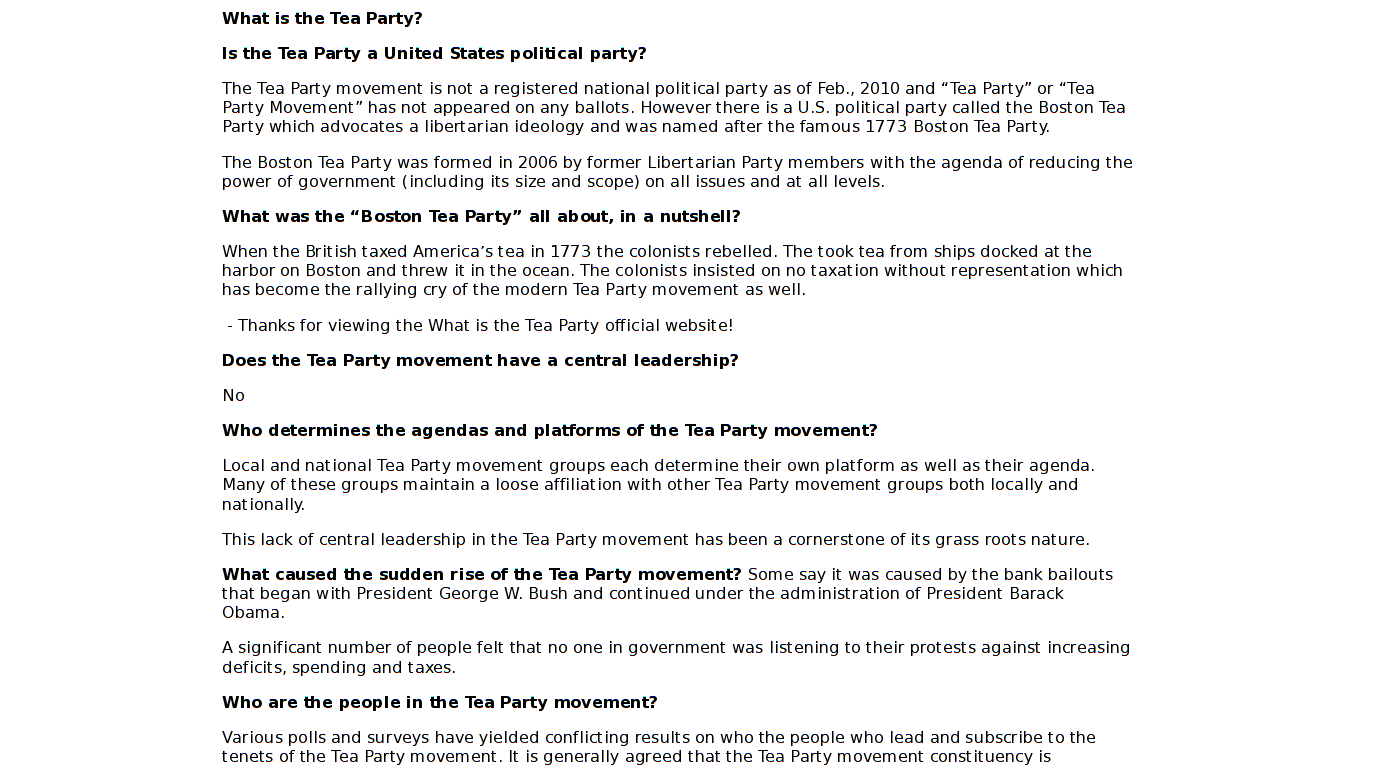
\includegraphics[height=\paperheight]{./presentation_images/TeaParty.png}
%       };
%     \end{tikzpicture}
%   \end{frame}
}


not the problem of 

For much of the social sciences, this is a fundamental problem. When we 


This is not just a problem of 

That's what I'm going to be talking about today, for a particular kind
of pattern: the urban neighborhood. Sociologists have been splitting up cities into neighborhoods for almost a hundred yearsWe have splitting up cities in




How could we convince ourselves that we have found a real pattern, that when we The problem 




 Since we know how the club did split, we
should not be all the impressed if someone can tune an algorithm to
split it up in a way that looks about right.





Given that we know what happened, 


My sense of what looks right is probably pretty similar to Especially for these smaller networks, 

With these algorithms, especially where you have a
relatively small network, it's pretty easy to push around the
output by adjusting parameters. 

This algorithm, on a particular run, came up with
this way of splitting things up. That output depended upon either the
user or the programmer adjusting one or more sensitivity threshold. If
the algorithm was run with other reasonable choices of parameters, it
might come up with a different way of splitting things up. Even if we weren't too worried about 
didn't, we saw in Jacob's presentation that there are different
approaches to community detection, and a different algorithm, that
seemed quite reasonable, might split things up differently.



 might have a set of algorithms that all appear equally reasonable ways of finding 






I want us to 



Let's say that we use 




There are many views about the uses of community detection. However,
as things stand now in the social sciences, we are not all that
interested in making more accurate predictions or for finding a more
concise representation of set of data. We like those things, but 

For us though,  but for social scientists
For social scientists, we will mainly be interested the community dect
One way of looking at the community detection algorithms that we have been talking about for the past two sessions

In the past few workshops, we have  this problem:




207
This is the introduction text. This text is not shown in the
presentation, but will be part of the article.

This text is once more not shown in the presentation.
\section{Main Part}
While this text is not shown in the presentation, the section command
also applies to the presentation.
We can add a subsection that is only part of the article like this:
\subsection<article>{Article-Only Section}
With some more text.
\begin{frame}
This text is part both of the article and of the presentation.
\begin{itemize}
\item This stuff is also shown in both version.
\item This too.
  \only<article>{\item This particular item is only part
    of the article version.}
\item<presentation:only@0> This text is also only part of the article.
\end{itemize}
\end{frame}

\end{document}